%\documentclass[10pt, xcolor=svgnames,trans]{beamer} % Para imprimir handouts
\documentclass[10pt,aspectratio=169]{beamer}  % Para imprimir presentación


% Color definitions, new environments and comands, packages
%%%%%%%%%%%%%%%%%%%%%%%%%%%%%%%%%%%%%%%%%%%%%%%%%%%%%%%%%%
%% Load packages
%%%%%%%%%%%%%%%%%%%%%%%%%%%%%%%%%%%%%%%%%%%%%%%%%%%%%%%%%%
\usepackage[spanish]{babel}
\usepackage{pgfpages}
\usepackage{booktabs}
\usepackage[scale=2]{ccicons}
\usepackage{appendixnumberbeamer}
\usepackage{enumitem}
\usepackage{mathtools}
\usepackage{datetime2}
\usepackage{environ}
\usepackage{amsmath}



%\renewcommand\pgfsetupphysicalpagesizes {\pdfpagewidth\pgfphysicalwidth\pdfpageheight\pgfphysicalheight}
%\pgfpagesuselayout{2 on 1}[a4paper,border shrink=5mm]


%%%%%%%%%%%%%%%%%%%%%%%%%%%%%%%%%%%%%%%%%%%%%%%%%%%%%%%%%%
%% New Environments and Commands
%%%%%%%%%%%%%%%%%%%%%%%%%%%%%%%%%%%%%%%%%%%%%%%%%%%%%%%%%%
\newcommand{\alertblue}[1]{%
{\setbeamercolor{alerted text}{fg = rb_blue}
\alert{#1}}
}

\newcommand{\alertred}[1]{%
{\setbeamercolor{alerted text}{fg = rb_red}
\alert{#1}}
}

\newcommand{\R}{\mathbb{R}}
\newcommand{\RN}{\mathbb{R}^n}
\newcommand{\RP}{\mathbb{R}_{+}}
\newcommand{\RNP}{\mathbb{R}^{n}_{+}}

\newcommand{\vx}{\mathbf{x}}
\newcommand{\vxe}{x_1, x_2, \dots, x_n}
\newcommand{\indi}{i = 1, 2, \dots, n}
\newcommand{\vsf}{\vspace{5pt}}


\newenvironment{varblock}[2]{%
  \setbeamercolor{block title}{#2}
  \begin{block}{#1}}{\end{block}}

\NewEnviron{myequation}{%
  \begin{equation*}
  \scalebox{1.5}{$\BODY$}
  \end{equation*}
  }

%%%%%%%%%%%%%%%%%%%%%%%%%%%%%%%%%%%%%%%%%%%%%%%%%%%%%%%%%%
%% Color Definitions
%%%%%%%%%%%%%%%%%%%%%%%%%%%%%%%%%%%%%%%%%%%%%%%%%%%%%%%%%%
% Bright Colors
\definecolor{br_blue}{HTML}{4477AA}
\definecolor{br_cyan}{HTML}{66CCEE}
\definecolor{br_green}{HTML}{228833}
\definecolor{br_yellow}{HTML}{CCBB44}
\definecolor{br_red}{HTML}{EE6677}
\definecolor{br_purple}{HTML}{AA3377}
\definecolor{br_grey}{HTML}{BBBBBB}

% Vibrant Colors
\definecolor{vi_blue}{HTML}{0077BB}
\definecolor{vi_cyan}{HTML}{33BBEE}
\definecolor{vi_teal}{HTML}{009988}
\definecolor{vi_orange}{HTML}{EE7733}
\definecolor{vi_red}{HTML}{CC3311}
\definecolor{vi_magenta}{HTML}{EE3377}
\definecolor{vi_grey}{HTML}{BBBBBB}

% Rainbow Colors
\definecolor{rb_red}{HTML}{E81416}
\definecolor{rb_orange}{HTML}{FFA500}
\definecolor{rb_yellow}{HTML}{FAEB36}
\definecolor{rb_green}{HTML}{79C314}
\definecolor{rb_blue}{HTML}{487DE7}
\definecolor{rb_indigo}{HTML}{4B369D}
\definecolor{rb_violet}{HTML}{70369D}

% Other colors
\definecolor{hi_yellow}{HTML}{DDAA33}
\definecolor{hi_red}{HTML}{BB5566}
\definecolor{hi_blue}{HTML}{004488}
\definecolor{dk_teal}{HTML}{23373B}
\definecolor{dk_orange}{HTML}{EB811B}


% Operadores matematicos
\DeclareMathOperator{\Hessian}{Hess}
\DeclareMathOperator*{\maxi}{Maximizar}


\usepackage{mathspec}

% Beamer Theme and Options
\usetheme[progressbar=foot,block=fill]{metropolis}
\setbeamercolor{progress bar}{fg=hi_blue, bg=hi_blue}


\usefonttheme{professionalfonts}
\setsansfont[BoldFont={Fira Sans}, Numbers={OldStyle}]{Fira Sans Light}
\setmathsfont(Digits)[Numbers={Lining, Proportional}]{Fira Sans Light}


% 
\title{Microeconomía I}
\subtitle{Preferencias y Posibilidades}
\date{Versión 0.1: \today}
\author{Santiago Foguet}
\institute{\textbf{Instituto de Investigaciones Económicas} \\ Facultad de Ciencias Económicas \\ Universidad Nacional de Tucumán}
\titlegraphic{\hfill
\includegraphics[height=.70cm]{images/logo_mod.jpg}}



\begin{document}

\maketitle

\begin{frame}{Tabla de Contenido}
  \setbeamertemplate{section in toc}[sections numbered]
  \tableofcontents[hideallsubsections]
\end{frame}


%%
% 
%%
\setbeamercolor{progress bar}{fg=rb_red, bg=rb_red}
\section{Introducción}
\setbeamercolor{frametitle}{bg=rb_red}


\begin{frame}{Modelo de Elección del Consumidor}

  Hay 4 elementos presentes en cualquier modelo de elección del consumidor:
  
  \begin{enumerate}[label=(\alph*)]
    \item El conjunto de consumo.
    \item El conjunto de consumo factible (o posible).
    \item La relación de preferencia.
    \item Supuestos sobre el comportamiento del consumidor.
\end{enumerate}

\end{frame}


\begin{frame}{Conjunto de Consumo}
	\alertred{Conjunto de Consumo}: $X$ representa el conjunto de todas las alternativas, o planes de consumo 
  completos, que el consumidor puede concebir, ya sea que algunas de ellas sean realizables en la práctica o no. 
  \vspace{5pt} \pause
  \begin{varblock}{Simbólicamente}{fg = vi_magenta}
	 $x_i$ representa el número de unidades del bien $i$ donde $x_i \in \RP$ y $\indi$.
   
   $\vx = \vec{x} = (\vxe)$ representa una cesta de consumo que contiene las distintas cantidades de los 
   $n$ diferentes bienes.
   
   $\vx \in X$ se representa por un punto $\vx \in \RNP$.
  \end{varblock}

\end{frame}
 
\begin{frame}{Conjunto de Consumo}
	\begin{alertblock}{Propiedades del Conjunto de Consumo}
    Los requisimos mínimos para el conjunto de consumo son:

    \begin{enumerate}
      \item $X \subseteq \RNP$.
      \item $X \text{es un conjunto cerrado}$.
      \item $X \text{es un conjunto convexo}$.
      \item $\mathbf{0} \in X$.
  \end{enumerate}
  \end{alertblock}
  \vspace{8pt}

  De ahora en más vamos a suponer por simplicidad que el conjunto de consumo coincidirá con todo
  el ortante no negativo, es decir, $X = \RNP$
\end{frame}

\begin{frame}{Conjunto de Consumo Factible}
	
  El \alertred{conjunto de consumo factible} $B$ representa aquellas alternativas o planes de consumo no solo 
  concebibles por el consumidor sino que además dadas las circunstancias del consumidor las mismas
  son alcanzables (o realizables).

  \begin{myequation}
    B \subset X
  \end{myequation}

\end{frame}


\setbeamercolor{progress bar}{fg=rb_orange, bg=rb_orange}
\section{Relación de Preferencia}
\setbeamercolor{frametitle}{bg=rb_orange}

\begin{frame}{Relaciones de Preferencia}
	\begin{varblock}{Preferencias del Consumidor}{fg = hi_blue}
	  \vsf
    Se representa con la \textit{relación binaria}, $\succsim$, definida sobre el conjunto 
    de consumo, $X$. Si $\vx^1 \succsim \vx^2$, diremos que $\vx^1 \text{ es al menos tan bueno como } \vx^2$
    para este consumidor.
    \vsf
  \end{varblock}
  \vspace{10pt}\pause
  \begin{varblock}{Axioma 1. Completitud}{fg = vi_teal}
    \vsf
	    Para todo $\vx^1$ y $\vx^2$ en $X$, será $\vx^1 \succsim \vx^2$ o $\vx^2 \succsim \vx^1$. 
    \vsf
  \end{varblock}
  \vspace{10pt} \pause
  \begin{varblock}{Axioma 2. Transitividad}{fg = vi_teal}
    \vsf
	    Para cualquiera tres cestas $\vx^1$, $\vx^2$ y $\vx^3$ en $X$, 
      si  $\vx^1 \succsim \vx^2$ y $\vx^2 \succsim \vx^3$ entonces $\vx^1 \succsim \vx^3$. 
    \vsf
  \end{varblock}

\end{frame}

\begin{frame}{Relaciones de Preferencia}
	\begin{varblock}{Relación de Preferencia}{fg = hi_blue}
	  \vsf
    La relación binaria, $\succsim$, sobre el conjunto de consumo $X$ se llama \alertblue{relación de preferencia}
    si cumple con los Axiomas 1 (Completitud) y 2 (Transitividad).
    \vsf
  \end{varblock}

\end{frame}


\begin{frame}{Relaciones de Preferencias}
  \begin{varblock}{Relación Estricta de Preferencia}{fg = hi_blue}
    \vsf
    La relación binaria $\succ$ sobre el conjunto de consumo $X$ definida por
    
    \[ \vx^1 \succ \vx^2 \quad \text{si y solo si} \quad \vx^1 \succsim \vx^2 \quad \text{and} \quad \vx^2 \succnsim  \vx^1\]

    se llama \alertblue{relación de preferencia estricta} y se lee como ``$\vx^1$ es estrictamente preferida a $\vx^2$''.
    \vsf
  \end{varblock}

\end{frame}


\begin{frame}{Relaciones de Preferencia}
  \begin{varblock}{Relación de Indiferencia}{fg = hi_blue}
    \vsf
    La relación binaria $\thicksim$ sobre el conjunto de consumo $X$ definida por
    
    \[ \vx^1 \thicksim \vx^2 \quad \text{si y solo si} \quad \vx^1 \succsim \vx^2 \quad \text{and} \quad \vx^2 \succsim  \vx^1\]

    se llama \alertblue{relación de indiferencia} y se lee como ``$\vx^1$ es indifirente a $\vx^2$''.
    \vsf
  \end{varblock}		

\end{frame}

\begin{frame}{Subconjuntos de Consumo definidos por la Relación de Preferencia}

  Sea $\vx^0$ cualquier punto en el conjunto de consumo, $X$. Relativo a este punto podemos definir los
  siguientes subconjuntos de $X$:

  \begin{enumerate}
    \item $\succsim(\vx^0) \equiv \{\vx \mid \vx \in X, \vx \succsim \vx^0\}$, llamdo el conjunto ``al menos tan bueno como''.
    \item $\precsim(\vx^0) \equiv \{\vx \mid \vx \in X, \vx^0 \succsim \vx\}$, llamdo el conjunto ``no mejor que''.
    \item $\prec(\vx^0) \equiv \{\vx \mid \vx \in X, \vx^0 \succ \vx\}$, llamdo el conjunto ``peor que''.
    \item $\succ(\vx^0) \equiv \{\vx \mid \vx \in X, \vx \succ \vx^0\}$, llamdo el conjunto ``mejor que''.
    \item $\thicksim(\vx^0) \equiv \{\vx \mid \vx \in X, \vx \thicksim \vx^0\}$, llamdo el conjunto ``de indiferencia''.
  \end{enumerate}

\end{frame}


\begin{frame}{Ejemplo con dos bienes}
  \centering
  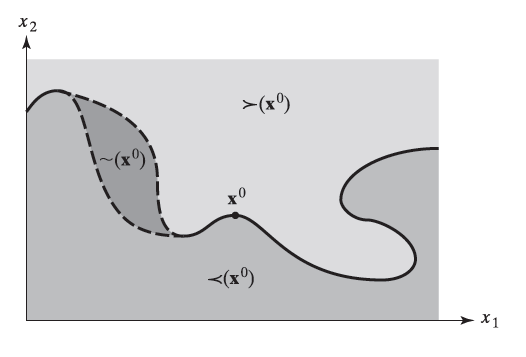
\includegraphics[scale=.70]{images/fig1.1.png}
\end{frame}

\begin{frame}{Axiomas adicionales}
	\begin{varblock}{Axioma 3. Continuidad}{fg = vi_teal}
    \vsf
      Para todo $\vx \in \RNP$, el conjunto ``al menos tan bueno como'', $\succsim(\vx)$, y el conjunto
      ``no mejor que'', $\precsim(\vx)$, son cerrados en $\RNP$. 
    \vsf
  \end{varblock}
  \pause
  \centering
  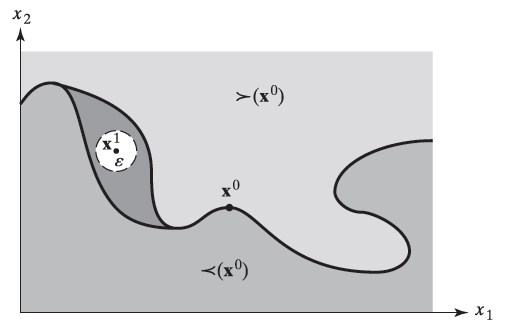
\includegraphics[scale=.50]{images/fig1.2.png}

\end{frame}


\begin{frame}{Axiomas adicionales}
	\begin{varblock}{Axioma 4'. No saciedad local}{fg = vi_teal}
    \vsf
      Para todo $\vx^0 \in \RNP$, y para todo $\varepsilon > 0$ existe algún $\vx \in B_\varepsilon(\vx^0) \cap \RNP$
      tal que $\vx \succ \vx^0$. 
    \vsf
  \end{varblock}
  \pause
  \centering
  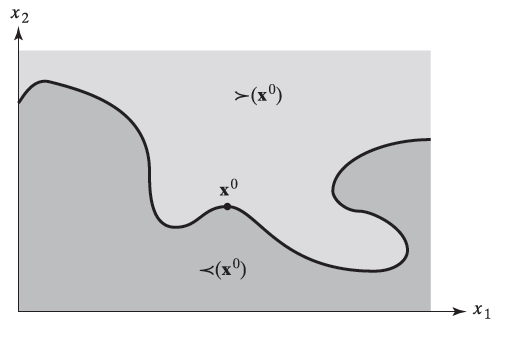
\includegraphics[scale=.50]{images/fig1.3.png}

\end{frame}

\begin{frame}{Axiomas adicionales}
	\begin{varblock}{Axioma 4. Monotonicidad estricta}{fg = vi_teal}
    \vsf
      Para todo $\vx^0, \vx^1 \in \RNP$, si $\vx^0 \geq \vx^1$ entonces $\vx^0 \succsim \vx^1$ mientras que 
      si $\vx^0 \gg \vx^1$ entonces $\vx^0 \succ \vx^1$.
    \vsf
  \end{varblock}
  \pause
  \centering
  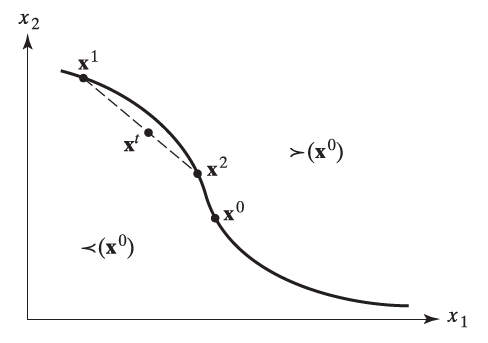
\includegraphics[scale=.50]{images/fig1.5.png}

\end{frame}

\begin{frame}{Axiomas adicionales}
	\begin{varblock}{Axioma 5'. Convexidad}{fg = vi_teal}
    \vsf
    Si  $\vx^0 \succsim \vx^1$ entonces $t \vx^1 + (1-t) \vx^0 \succsim \vx^0 $ para todo $t \in [0,1]$
    \vsf
  \end{varblock}

\end{frame}

\begin{frame}{Axiomas adicionales}
	\begin{varblock}{Axioma 5. Convexidad Estricta}{fg = vi_teal}
    \vsf
    Si  $\vx^0 \neq  \vx^1$ y $\vx^0 \succsim \vx^1$ entonces $t \vx^1 + (1-t) \vx^0 \succsim \vx^0 $ para todo $t \in (0,1)$
    \vsf
  \end{varblock}
  \pause
  \centering
  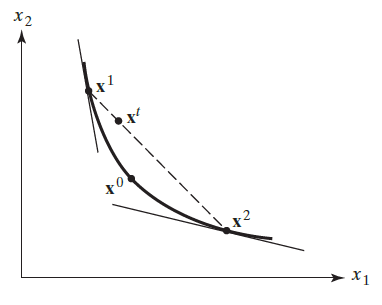
\includegraphics[scale=.60]{images/fig1.6.png}

\end{frame}


\setbeamercolor{progress bar}{fg=rb_yellow, bg=rb_yellow}
\section{Función de Utilidad}
\setbeamercolor{frametitle}{fg = black, bg=rb_yellow}

\begin{frame}{Función de Utilidad}
	
  \begin{varblock}{Función de Utilidad que Representa la Relación de Preferencia}{fg = vi_magenta}
    \vsf
	  Una función real $U: \RNP \rightarrow \R$ se llama función de utilidad que representa la
    relación de preferencia, $\succsim $, si para todo $\vx^0, \vx^1 \in \RNP$, $U(\vx^0) \geq U(\vx^1)
    \Longleftrightarrow \vx^0 \succsim \vx^1$
    \vsf
  \end{varblock}
\vspace{10pt} \pause
  \begin{varblock}{Teorema 1. Existencia de una Función Real que represente $\succsim $}{fg = vi_orange}
    \vsf
	  Si la relación binaria $\succsim $ es completa, transivita, continua y estrictamente monotónica entonces
    existe una función real continua $U: \RNP \rightarrow \R$ la cual representa a $\succsim$.
    \vsf
  \end{varblock}

\end{frame}

\begin{frame}{Función de Utilidad}
  \begin{varblock}{Teorema 2. Invariancia de la Función de Utilidad }{fg = vi_orange}
    \vsf
	  Sea $\succsim $ la relación de preferencia en $\RNP$ y suponga que $U(\vx)$ es una función de utilidad que
    representa esa relación. Entonces $V(\vx)$ también representa a $\succsim$ si y solo si $V(\vx) = f(U(\vx))$
    para cada $\vx$, donde $f: \R \rightarrow \R$ es estrictamente creciente en el conjunto de valores 
    adoptados por $U$.
    \vsf
  \end{varblock}
\pause
  \begin{varblock}{Teorema 3. Propiedades de las Preferencias y Función de Utilidad }{fg = vi_orange}
    \vsf
    Sea $\succsim $ representada por $U: \RNP \rightarrow \R$. Entonces:
    \begin{enumerate}
      \item $U(\vx)$ es estrictamente creciente si y solo si $\succsim$ es estrictamente monotonica.
      \item $U(\vx)$ es cuasicóncava si y solo si $\succsim$ es convexa.
      \item $U(\vx)$ es estrictamente cuasicóncava si y solo si $\succsim$ es estrictamente convexa.
    \end{enumerate}
    \vsf
  \end{varblock}

  \end{frame}



  \setbeamercolor{progress bar}{fg=rb_green, bg=rb_green}
  \section{Conjunto de Consumo Factible}
  \setbeamercolor{frametitle}{fg = white, bg=rb_indigo}




%------------------------------------------------------
% Varios
%------------------------------------------------------
\setbeamercolor{progress bar}{fg=rb_violet, bg=rb_violet}
\section{Bibliografía}
\setbeamercolor{frametitle}{bg=rb_indigo}

\nocite{*}
\begin{frame}[allowframebreaks]
\frametitle{Bibliografía}
    {%\footnotesize
    \bibliographystyle{chicago}
    \bibliography{biblio}
   }
\end{frame}


%% Licencia de uso de la presentación
\metroset{numbering=none}
{\setbeamercolor{palette primary}{fg=white, bg=rb_indigo}
\begin{frame}[standout]
	This presentation is licensed under a
	\href{https://creativecommons.org/licenses/by-nc-sa/4.0/}{Creative Commons Attribution-NonCommercial-ShareAlike 4.0 International}.
	
	\begin{center}
		\ccbyncsa
	\end{center}
\end{frame}
}


\end{document}
